\documentclass[journal]{IEEEtran}

%----------------------------------------------------------------------------------------
% PACKAGES
%----------------------------------------------------------------------------------------
\usepackage{amsmath,amsfonts}
\usepackage{algorithmic}
\usepackage{algorithm}
\usepackage{array}
\usepackage[font=normalsize,labelfont=sf,textfont=sf]{subfig}
\usepackage{textcomp}
\usepackage{stfloats}
\usepackage{url}
\usepackage{verbatim}
\usepackage{graphicx}
\usepackage{cite}
\hyphenation{op-tical net-works semi-conduc-tor IEEE-Xplore}
\usepackage[
    colorlinks=true, 
    linkcolor=blue, 
    citecolor=blue,
    urlcolor=blue
]{hyperref}

%----------------------------------------------------------------------------------------
% DOCUMENT BODY
%----------------------------------------------------------------------------------------
\begin{document}

\title{Dynamic Scene Modeling and Rendering: A Survey of Methods and Applications}

\author{
  Yuwei~Zhao$^{1,2}$,
  Kaiyuan~Zhang$^{1,2}$,
  Yuxiang~Liu$^{1,2}$,
  Yilin~Zhang$^{1,2}$,
  and~Keqin~Zhang$^{1,2}$
\thanks{$^{1}$School of Computer Science and Technology, Ocean University of China, Qingdao 266100, China.}
\thanks{$^{2}$School of MPs \& EPs, Heriot-Watt University, Edinburgh EH14 4AS, UK.}
}

\maketitle

%----------------------------------------------------------------------------------------
\begin{abstract}
  Dynamic scene modeling and reconstruction from video streams have witnessed a paradigm shift with the advent of Neural Radiance Fields (NeRF) and 3D Gaussian Splatting (3DGS). 
  While NeRF-based methods offer photorealistic quality via implicit neural representations, they often suffer from prohibitive training and rendering costs. 
  Recently, 3DGS has emerged as a powerful alternative, enabling real-time rendering through explicit splatting techniques, though it introduces new challenges regarding storage overhead and temporal consistency. 
  In this paper, we present a comprehensive survey of video-based 3D reconstruction methods, categorizing them into implicit and explicit approaches. 
  We systematically evaluate their trade-offs in terms of rendering quality, speed, and memory consumption across diverse scenarios. 
  Furthermore, we summarize the limitations of current state-of-the-art methods and discuss future directions. 
  Our compiled resources and code are available at \url{https://github.com/8arbatos/Academic-English-Group-Paper}.
\end{abstract}

%----------------------------------------------------------------------------------------
\begin{IEEEkeywords}
  3D Reconstruction, Dynamic Scene Modeling, Neural Radiance Fields (NeRF), Gaussian Splatting, Novel View Synthesis, Survey.
\end{IEEEkeywords}

%----------------------------------------------------------------------------------------
\section{Introduction}
\IEEEPARstart{W}{ith} the rapid advancement of virtual reality (VR), augmented reality (AR), and the Metaverse, the demand for photorealistic 3D content creation has surged exponentially. 
Dynamic scene modeling, which aims to reconstruct 3D geometry and appearance from 2D video streams, serves as a fundamental technology for these applications, enabling immersive telepresence, free-viewpoint video, and digital human avatars \cite{intro_metaverse}. 
Unlike static scene reconstruction, modeling dynamic scenes from video presents a highly ill-posed inverse problem due to the entanglement of object motion, topology changes, and time-variant lighting conditions.

%----------------------------------------------------------------------------------------
\begin{figure}[!t]
  \centering
  \includegraphics[width=\linewidth]{./img/3d_reconstruction_benchmark.png} 
  \caption{Performance landscape of video-based 3D reconstruction methods. We visualize the trade-off between rendering speed (FPS, log scale) and reconstruction quality (PSNR). Implicit methods achieve high quality but slow inference. Explicit methods (3DGS) achieve real-time performance while maintaining high fidelity.}
  \label{fig:teaser_landscape}
\end{figure}

%----------------------------------------------------------------------------------------
Traditionally, 3D reconstruction relied on Structure-from-Motion (SfM) and Multi-View Stereo (MVS) algorithms \cite{colmap}. 
While these methods, such as COLMAP, provide robust camera pose estimation, they struggle to capture thin structures and view-dependent effects (e.g., reflections). 
More importantly, traditional pipelines typically assume a static world, making them brittle when applied to dynamic video sequences where geometry consistency is violated over time.

The field witnessed a paradigm shift with the introduction of \textbf{Neural Radiance Fields (NeRF)} \cite{nerf}. 
By representing scenes as implicit continuous functions parameterized by Multi-Layer Perceptrons (MLPs), NeRF achieved unprecedented rendering quality. 
Subsequent works, such as D-NeRF \cite{dnerf} and Nerfies \cite{nerfies}, extended this implicit paradigm to dynamic domains by introducing deformation fields to handle non-rigid motion. 
However, implicit methods suffer from prohibitive computational costs due to the extensive ray-marching sampling required during both training and inference, limiting their deployment in real-time applications.

Recently, \textbf{3D Gaussian Splatting (3DGS)} \cite{gaussian_splatting} has emerged as a compelling alternative, marking a return to explicit volumetric representations. 
By combining the differentiability of deep learning with the efficiency of rasterization-based rendering, 3DGS enables real-time rendering (100+ FPS) and fast training speeds. 
This breakthrough has triggered a new wave of research focused on extending Gaussian primitives to 4D spatiotemporal modeling \cite{4dgs, dynamic3dgs}, aiming to combine the efficiency of explicit representations with the flexibility of neural fields.

%----------------------------------------------------------------------------------------
\begin{figure*}[!t]
  \centering
  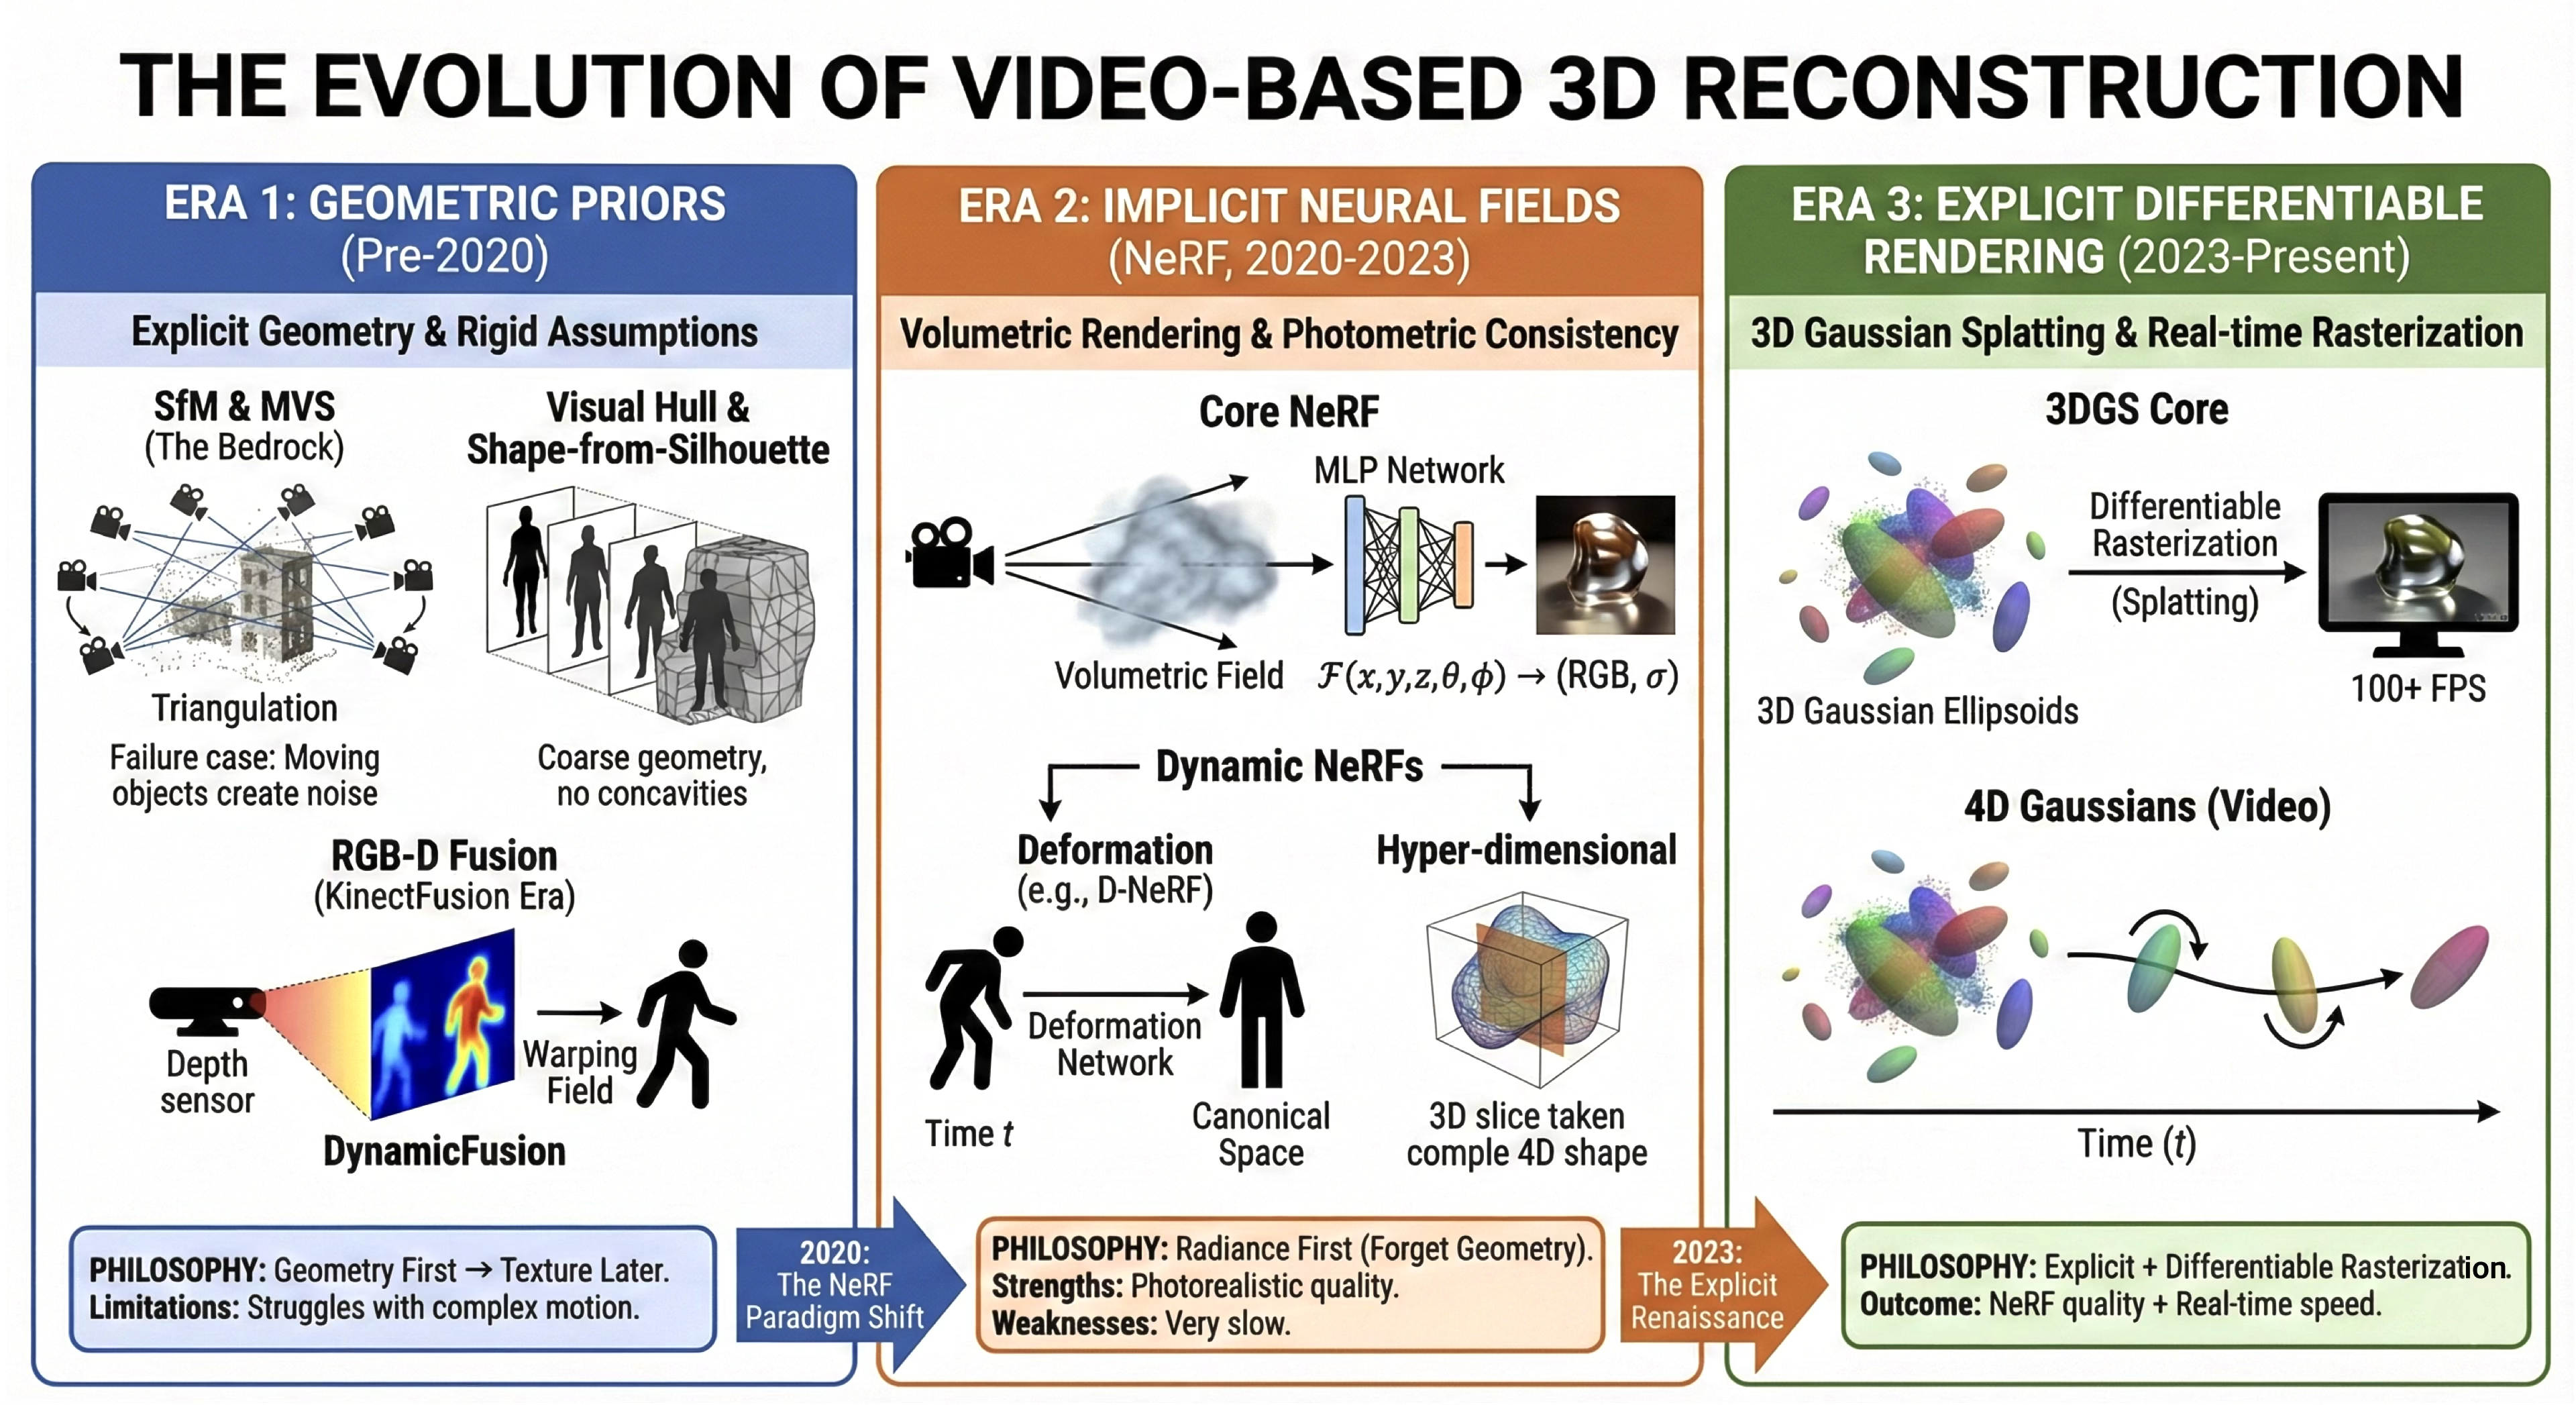
\includegraphics[width=0.95\textwidth]{./img/3d_reconstruction_evolution.png}
  \caption{Visualization of the evolution of video-based 3D reconstruction}
  \label{fig:evolution_3d_reconstruction}
\end{figure*}

%----------------------------------------------------------------------------------------
Despite the explosion of research papers in this domain, a systematic comparison between implicit (NeRF-based) and explicit (Gaussian-based) approaches for video modeling is lacking. 
In this survey, we provide a comprehensive review of the state-of-the-art methods for video-based 3D reconstruction. 
The main contributions of this paper are summarized as follows:

\begin{itemize}
  \item We propose a structured taxonomy of dynamic scene modeling methods, categorizing them into \textit{Deformation-based}, \textit{Spacetime-based}, and \textit{Hybrid} approaches across both implicit and explicit representations.
  \item We provide an in-depth analysis of the transition from NeRF to 3D Gaussian Splatting, highlighting the trade-offs between rendering quality, training efficiency, and storage overhead.
  \item We conduct a comparative evaluation of representative frameworks and discuss open challenges, including storage optimization and long-duration video modeling, to guide future research directions.
\end{itemize}

%----------------------------------------------------------------------------------------
\section{Preliminaries}
In this section, we first provide a unified mathematical formulation for the problem of video-based 3D reconstruction. 
We then detail the fundamental principles of the two dominant paradigms: the implicit neural representation introduced by NeRF and the explicit differentiable representation proposed by 3D Gaussian Splatting.

%----------------------------------------------------------------------------------------
\subsection{Mathematical Formulation}
Video-based 3D reconstruction can be fundamentally formulated as an inverse rendering problem. 
Given a sequence of $N$ observed images $\mathcal{I} = \{I_1, I_2, \dots, I_N\}$ captured from a video stream, along with their corresponding camera poses $\mathcal{P} = \{P_1, P_2, \dots, P_N\}$ (typically estimated via Structure-from-Motion, SfM), 
the goal is to optimize a 3D scene representation $\mathcal{S}$ such that it can synthesize novel views consistent with the input observations.

Formally, we seek to minimize the photometric reconstruction error between the rendered images and the ground truth images:
\begin{equation}
  \mathcal{S}^* = \mathop{\arg\min}_{\mathcal{S}} \sum_{k=1}^{N} \mathcal{L} \left( \mathcal{R}(\mathcal{S}, P_k), I_k \right)
\end{equation}
where $\mathcal{R}(\cdot)$ denotes the differentiable rendering function that projects the 3D representation $\mathcal{S}$ onto the 2D image plane given a camera pose $P_k$, 
and $\mathcal{L}$ represents the loss function (typically $\ell_1$, $\ell_2$, or D-SSIM) measuring the discrepancy between the synthesized and observed pixels.

%----------------------------------------------------------------------------------------
\subsection{Fundamentals of Neural Radiance Fields}
Neural Radiance Fields (NeRF) represent a scene implicitly as a continuous volumetric function parameterized by a Multi-Layer Perceptron (MLP).

%----------------------------------------------------------------------------------------
\subsubsection{Scene Representation}
The core function, denoted as $F_{\Theta}$, maps a continuous 5D coordinate input---consisting of a 3D spatial location $\mathbf{x} = (x, y, z)$ and
 a 2D viewing direction $\mathbf{d} = (\theta, \phi)$---to a volume density $\sigma$ and a view-dependent emitted color $\mathbf{c} = (r, g, b)$:
\begin{equation}
  F_{\Theta}: (\mathbf{x}, \mathbf{d}) \to (\mathbf{c}, \sigma)
\end{equation}
By conditioning the color on the viewing direction $\mathbf{d}$, NeRF is able to model complex view-dependent effects such as specular reflections.

%----------------------------------------------------------------------------------------
\subsubsection{Volume Rendering Equation}
To synthesize an image, NeRF employs classical volume rendering techniques. 
The color $C(\mathbf{r})$ of a camera ray $\mathbf{r}(t) = \mathbf{o} + t\mathbf{d}$ is computed by integrating the radiance along the ray from near bound $t_n$ to far bound $t_f$:
\begin{equation}
  C(\mathbf{r}) = \int_{t_n}^{t_f} T(t) \sigma(\mathbf{r}(t)) \mathbf{c}(\mathbf{r}(t), \mathbf{d}) \, dt
\end{equation}
where $T(t)$ denotes the accumulated transmittance, representing the probability that the ray travels from $t_n$ to $t$ without hitting any other particles:
\begin{equation}
  T(t) = \exp \left( -\int_{t_n}^{t} \sigma(\mathbf{r}(s)) \, ds \right)
\end{equation}

%----------------------------------------------------------------------------------------
\subsubsection{Discretization}
In practice, the continuous integral is approximated using stratified sampling. The ray is divided into $N$ bins, and the integral is reduced to a finite sum:
\begin{equation}
  \begin{split}
    \hat{C}(\mathbf{r}) &= \sum_{i=1}^{N} T_i (1 - \exp(-\sigma_i \delta_i)) \mathbf{c}_i\,, \\
    & \text{where } T_i = \exp \left( -\sum_{j=1}^{i-1} \sigma_j \delta_j \right)
  \end{split}
\end{equation}
Here, $\delta_i$ is the distance between adjacent samples. This differentiable rendering pipeline allows the MLP parameters $\Theta$ to be optimized via stochastic gradient descent.

%----------------------------------------------------------------------------------------
\subsection{Fundamentals of 3D Gaussian Splatting}
To address the computational inefficiency of volumetric ray-marching in NeRF, 3D Gaussian Splatting (3DGS) introduces an explicit representation based on anisotropic 3D Gaussians, 
enabling real-time rendering via rasterization.

%----------------------------------------------------------------------------------------
\subsubsection{3D Gaussian Representation}
The scene is represented by a set of 3D Gaussians. Each primitive is defined by a center position $\mu$, a covariance matrix $\Sigma$, an opacity $\alpha$, 
and spherical harmonics (SH) coefficients for view-dependent color. The influence of a Gaussian at a point $\mathbf{x}$ is defined as:
\begin{equation}
  G(\mathbf{x}) = \exp \left( -\frac{1}{2} (\mathbf{x} - \mu)^T \Sigma^{-1} (\mathbf{x} - \mu) \right)
\end{equation}
To ensure the covariance matrix $\Sigma$ remains positive semi-definite during optimization, it is factorized into a scaling matrix $S$ and a rotation matrix $R$:
\begin{equation}
  \Sigma = R S S^T R^T
\end{equation}

%----------------------------------------------------------------------------------------
\subsubsection{Projection and Splatting}
Unlike NeRF's ray-marching, 3DGS projects the 3D Gaussians directly onto the 2D image plane. Given a viewing transformation $W$, the covariance matrix $\Sigma'$ in camera coordinates is approximated as:
\begin{equation}
  \Sigma' = J W \Sigma W^T J^T
\end{equation}
where $J$ is the Jacobian of the affine approximation of the projective transformation. This step effectively "splats" the 3D ellipsoids into 2D ellipses.

%----------------------------------------------------------------------------------------
\subsubsection{Tile-based Blending}
The final pixel color is computed using $\alpha$-blending of the $N$ sorted Gaussians overlapping the pixel:
\begin{equation}
  C = \sum_{i \in \mathcal{N}} c_i \alpha_i \prod_{j=1}^{i-1} (1 - \alpha_j)
\end{equation}
Here, $\alpha_i$ is obtained by evaluating the 2D Gaussian multiplied by the learned opacity. 
This tile-based rasterization approach allows for highly efficient backpropagation and real-time rendering speeds ($>100$ FPS), making it particularly suitable for high-resolution video reconstruction.

%----------------------------------------------------------------------------------------
\section{Taxonomy of Dynamic Scene Modeling} % Core

%----------------------------------------------------------------------------------------
\subsection{Implicit Deformation Fields}
This category of methods addresses dynamic scene modeling by decoupling the scene's geometry into two components: a static structure and a time-variant deformation.

%----------------------------------------------------------------------------------------
\begin{figure}[!t]
  \centering
  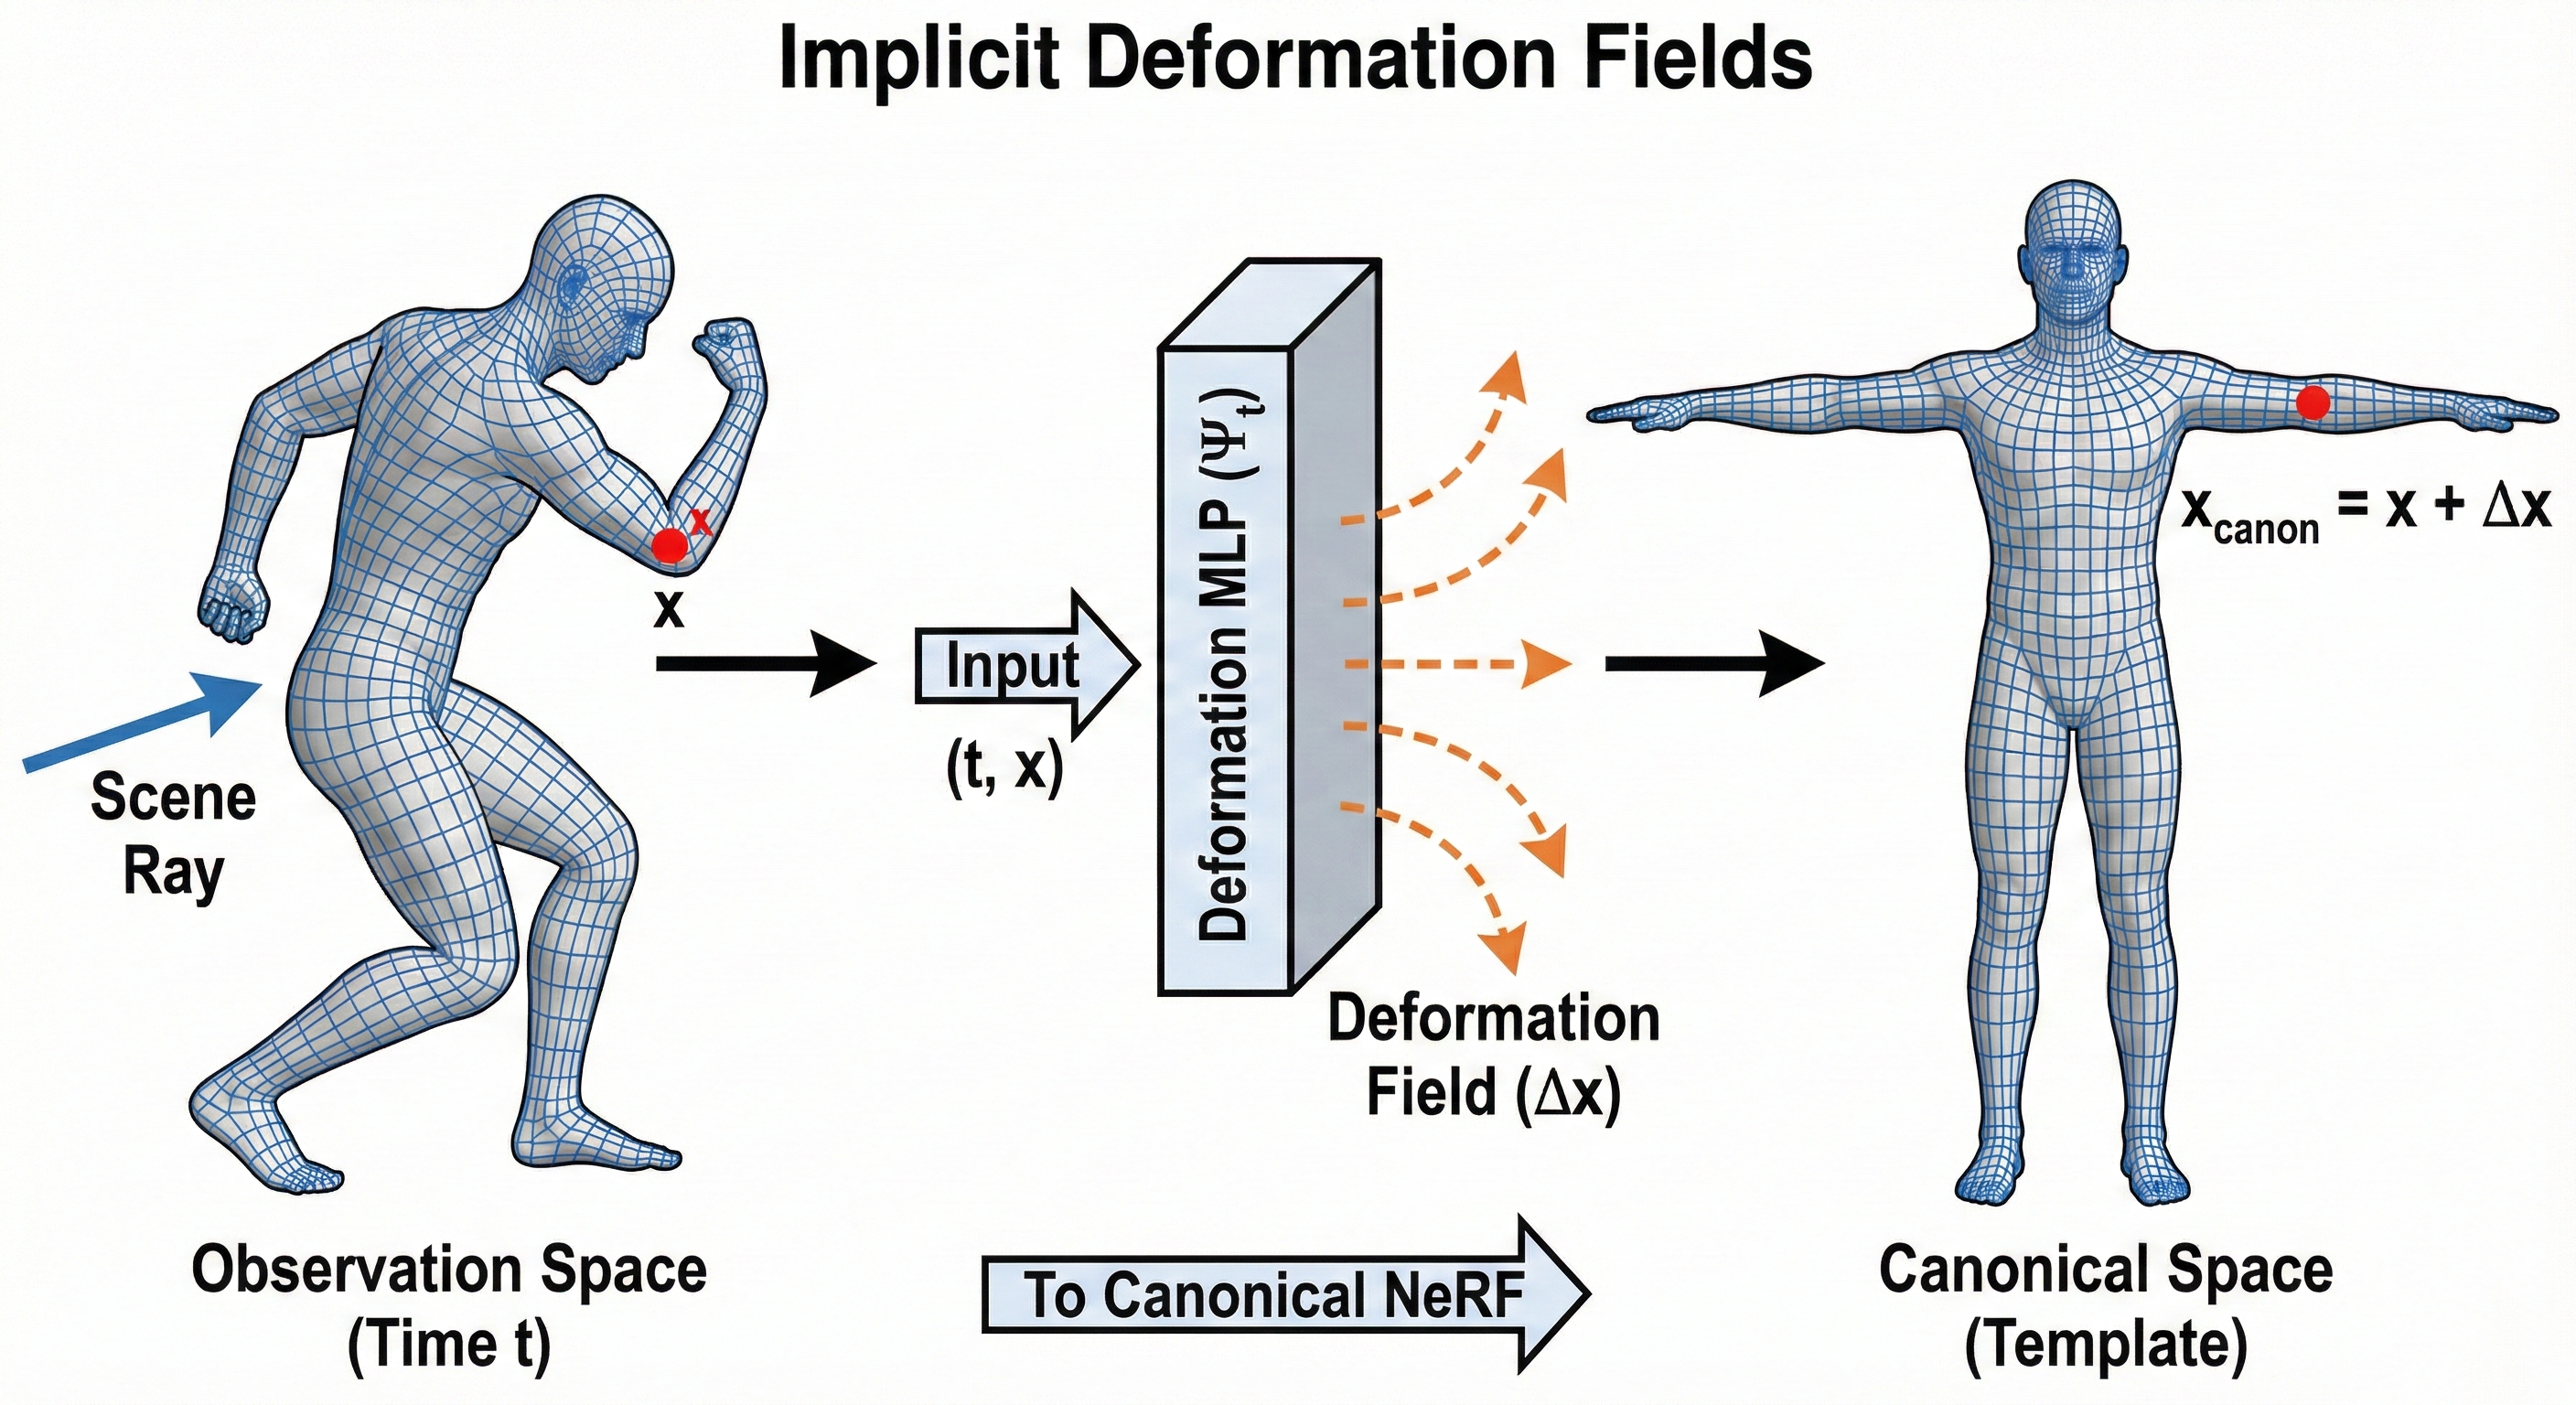
\includegraphics[width=\linewidth]{./img/implicit_deformation_fields.png}
  \caption{Overview of Implicit Deformation Fields. Dynamic scenes are modeled by learning a deformation field that maps points from the observation space to a canonical space, where a static NeRF represents the scene's appearance and geometry.}
  \label{fig:implicit_deformation_fields}
\end{figure}

%----------------------------------------------------------------------------------------
\subsubsection{Core Assumption and Architecture}
The fundamental assumption of this paradigm is the existence of a time-independent \textbf{Canonical Space}. 
The dynamic scene observed at any time instance $t$ is modeled as a warped version of this canonical configuration \cite{dnerf}. 
This approach simplifies the learning objective by separating motion from appearance.

Architecturally, these frameworks typically employ two joint Multilayer Perceptrons (MLPs):
\begin{itemize}
  \item \textbf{Deformation Network:} This network learns the mapping from the observation space to the canonical space. 
  It takes the current 3D position $\mathbf{x}$ and a temporal indicator (time $t$ or a latent code $\omega_i$) as input, and outputs a displacement vector $\Delta \mathbf{x}$ (or a dense vector field).

  \item \textbf{Canonical Network:} This is a standard static NeRF that represents the scene in its ``rest pose''. 
  It takes the corrected position $\mathbf{x}_{canon} = \mathbf{x} + \Delta \mathbf{x}$ and viewing direction $\mathbf{d}$ to predict color $\mathbf{c}$ and density $\sigma$.
\end{itemize}

Mathematically, this process can be formulated as:
\begin{equation}
  (\mathbf{x}_{canon}, \Delta \mathbf{x}) = \mathcal{D}(\mathbf{x}, t), \quad (\mathbf{c}, \sigma) = \mathcal{F}_{\text{NeRF}}(\mathbf{x}_{canon}, \mathbf{d})
\end{equation}
where $\mathcal{D}$ represents the deformation network and $\mathcal{F}_{\text{NeRF}}$ represents the canonical radiance field \cite{dnerf}.

%----------------------------------------------------------------------------------------
\subsubsection{Representative Frameworks}
The evolution of implicit deformation fields can be traced through three milestone works, each addressing specific limitations of the previous:

\textbf{D-NeRF:} Pumarola et al.  established the baseline for this category by introducing the translation field $\mathbf{x}(t) \to \mathbf{x}_{canon} + \Delta \mathbf{x}$. 
D-NeRF optimizes the scene using a sparse set of monocular images, successfully reconstructing non-rigid objects (e.g., a moving mechanical arm or a jumping human) by learning a continuous displacement field conditioned on time $t$ \cite{dnerf}.

\textbf{Nerfies:} While D-NeRF works well for synthetic or controlled data, applying this concept to casual selfie videos introduces challenges such as camera movement and under-constrained deformations. 
Park et al.  introduced \textit{Nerfies}, which replaces the explicit time input $t$ with learned latent deformation codes $\omega_i$ to handle irregular timestamps. 
Crucially, Nerfies introduces \textbf{elastic regularization} (based on the Jacobian of the deformation field) to impose rigidity priors. This prevents the ``background'' or ``rigid parts'' of a face from distorting unrealistically, ensuring that the deformation field remains plausible even with sparse views \cite{nerfies}.

\textbf{HyperNeRF:} A critical limitation of pure deformation fields is their continuity; they cannot model \textbf{topological changes} (e.g., a mouth opening/closing or separating objects) because mapping a continuous space to a discontinuous one requires a break in the vector field \cite{hypernerf}. 
Park et al.  proposed \textit{HyperNeRF} to address this by lifting the scene into a higher-dimensional ``hyperspace''. Instead of simply deforming points, HyperNeRF learns a \textbf{slicing surface} in this ambient hyperspace. 
Topological variations are effectively modeled as continuous deformations of the slicing manifold, allowing the method to handle complex level-set changes that D-NeRF and Nerfies cannot \cite{hypernerf}.

%----------------------------------------------------------------------------------------
\subsubsection{Summary}
\begin{itemize}
  \item \textbf{Pros}: These methods excel at reconstructing non-rigid, organic objects (such as human faces and bodies) with photorealistic quality, inheriting the high-frequency detail capabilities of the underlying NeRF representation \cite{nerf}.
  \item \textbf{Cons}: The primary drawback is the computational cost; training is extremely slow due to the MLP queries required for ray marching. 
\end{itemize}
Furthermore, pure deformation-based methods (excluding HyperNeRF) fundamentally struggle with large topological changes due to the continuity constraints of neural networks \cite{hypernerf}.

%----------------------------------------------------------------------------------------
\subsection{Spacetime Neural Fields}
Unlike deformation-based methods that warp a static template, Spacetime Neural Fields treat time as an intrinsic dimension of the scene. 
These methods directly learn a continuous function over the spatiotemporal domain, effectively slicing the 4D volume to retrieve the state of the scene at any specific moment.

%----------------------------------------------------------------------------------------
\subsubsection{Core Concepts and Architecture}
The fundamental shift in this paradigm is the expansion of the input domain. 
While a standard NeRF maps a 5D coordinate $(\mathbf{x}, \mathbf{d})$ to color and density, Spacetime Neural Fields extend this to a \textbf{Higher-dimensional Input} by incorporating time $t$. 
The mapping function evolves into $F_{\Theta}: (\mathbf{x}, \mathbf{d}, t) \to (\mathbf{c}, \sigma)$. To handle complex dynamics, two primary strategies are employed:

\textbf{Latent Code Modulation:} Instead of using a raw scalar $t$, methods like DyNeRF learn a set of compact, time-variant \textit{latent codes} $\mathbf{z}_t$ for each frame. 
These codes are fed into the MLP alongside spatial coordinates, acting as a switch that modulates the network's activations to represent topological changes, varying illumination, and transient objects.

\textbf{Physical Consistency (Scene Flow):} To enforce temporal coherence, some approaches incorporate physical constraints. 
A notable example is \textbf{NSFF (Neural Scene Flow Fields)} \cite{nsff}, which predicts not only the radiance and density but also the 3D \textit{Scene Flow} vector $\mathbf{f}$. 
By enforcing consistency between the backward/forward flow and the geometric positions across frames, the model ensures that the dynamic representation adheres to physical motion laws.

Mathematically, the general formulation for this category can be expressed as:
\begin{equation}
    (\mathbf{c}, \sigma) = F_{\Theta}(\mathbf{x}, \mathbf{d}, \mathbf{z}_t) \quad \text{or} \quad (\mathbf{c}, \sigma, \mathbf{f}) = F_{\Theta}(\mathbf{x}, t)
\end{equation}
where $\mathbf{z}_t$ represents the learned latent code and $\mathbf{f}$ denotes the predicted scene flow vector.

%----------------------------------------------------------------------------------------
\subsubsection{Representative Frameworks}
In the following, we discuss two representative frameworks that address dynamic modeling under distinct input constraints: \textbf{DyNeRF} for synchronized multi-view videos and \textbf{Video-NeRF} for casual monocular captures.

\textbf{DyNeRF (Dynamic NeRF):} Li et al. proposed DyNeRF to address the challenge of reconstructing dynamic scenes from multi-view videos \cite{dynerf}. 
Instead of a deformation field, DyNeRF conditions the radiance field on a learnable latent embedding $\mathbf{z}_t$. This allows the model to capture complex dynamics that are difficult to model with continuous deformations, such as flame, pouring liquid (topology changes), and view-dependent lighting effects.

\textbf{Video-NeRF:} Focusing on the challenging monocular setting, Video-NeRF learns a direct mapping from spacetime coordinates $(\mathbf{x}, t)$ to an irradiance field (omitting view dependence to handle single-video ambiguity). 
To prevent the ``motion-appearance ambiguity'' (where geometry changes are incorrectly explained as texture changes), it incorporates depth supervision from pre-trained monocular estimators and introduces a ``static scene loss'' to constrain unobserved regions by propagating information across time \cite{video_nerf}.

%----------------------------------------------------------------------------------------
\subsubsection{Summary}
\begin{itemize}
  \item \textbf{Pros:} These methods are well-suited for large-scale scenes and complex dynamics involving drastic topological changes (e.g., fluid dynamics, fire) where defining a canonical template is infeasible.
  \item \textbf{Cons:} The addition of the time dimension significantly expands the sampling space, leading to the ``curse of dimensionality''. Without sufficient data (e.g., multi-view rigs) or strong regularization (e.g., depth/flow priors), these models are prone to overfitting or producing temporally incoherent artifacts.
\end{itemize}

%----------------------------------------------------------------------------------------
\subsection{Dynamic Gaussian Splatting}
This category represents the current state-of-the-art (SOTA), marking a shift from implicit neural fields back to explicit, rasterizable primitives. By extending 3D Gaussian Splatting (3DGS) to the temporal domain, these methods aim to combine the photorealism of NeRF with the real-time rendering capabilities of rasterization.

%----------------------------------------------------------------------------------------
\subsubsection{Core Concepts and Architecture}
The fundamental primitive in this paradigm is the \textbf{3D Gaussian}, characterized by a center position $\mu$, a covariance matrix $\Sigma$, an opacity $\alpha$, and spherical harmonics (SH) for color. To ensure physical validity, the covariance is factorized into scaling $S$ and rotation $R$ matrices: $\Sigma = R S S^T R^T$.

To handle dynamic scenes without incurring the prohibitive memory cost of storing per-frame Gaussians, the core strategy is \textbf{Temporal Parameterization}. The attributes of Gaussians are modeled as functions of time $t$. The influence of a dynamic Gaussian at time $t$ is formulated as:
\begin{equation}
    G(\mathbf{x}, t) = \exp \left( -\frac{1}{2} (\mathbf{x} - \mu(t))^T \Sigma(t)^{-1} (\mathbf{x} - \mu(t)) \right)
\end{equation}
where $\mu(t)$ and $\Sigma(t)$ denote time-variant position and covariance. Two primary streams exist to model these functions:

\textbf{Deformation-based Approach:} Similar to D-NeRF, this stream maintains a set of static \textit{Canonical Gaussians}. A learnable deformation network predicts offsets for position, rotation, and scaling ($\delta x, \delta r, \delta s$) to warp canonical primitives to the current timestamp.

\textbf{4D Spacetime Primitives:} Alternatively, the scene can be represented holistically by querying a high-dimensional feature space. Techniques like \textbf{HexPlane decomposition} factorize the 4D spatiotemporal volume into multi-resolution 2D planes (e.g., $xy, xt, yt$) to efficiently encode temporal dynamics.

%----------------------------------------------------------------------------------------
\begin{figure}[!t]
  \centering
  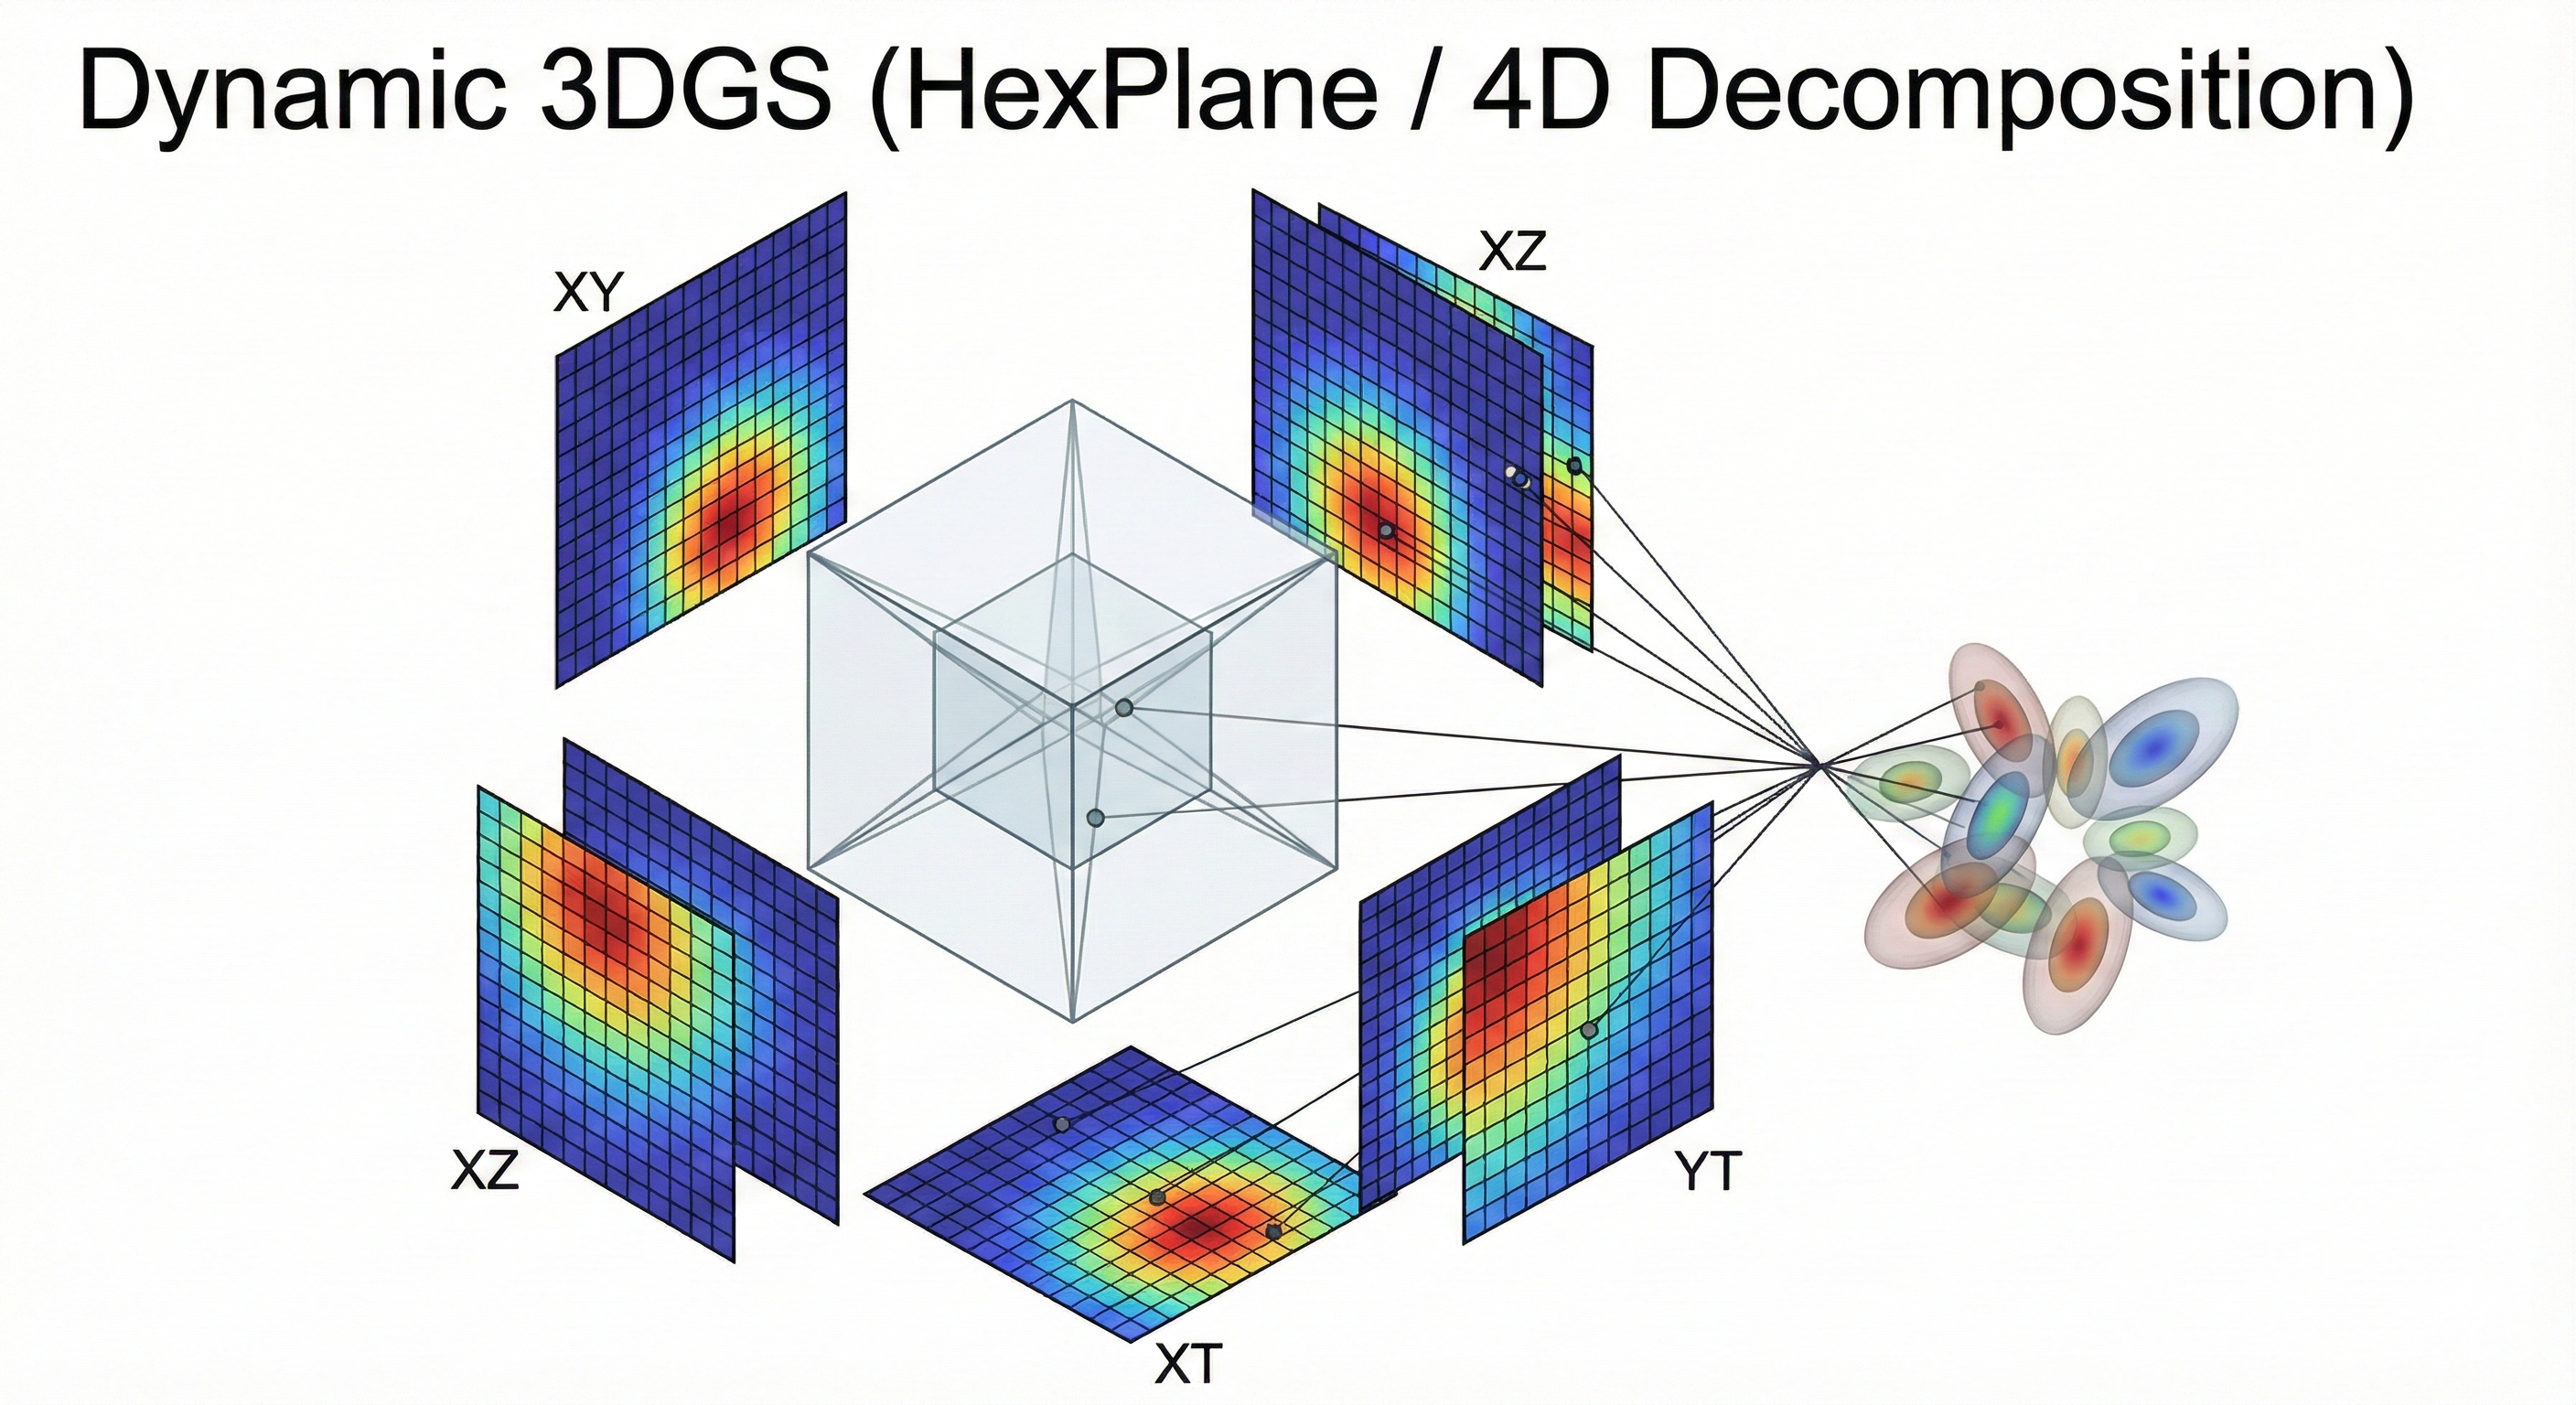
\includegraphics[width=\linewidth]{./img/dynamic_gs.png}
  \caption{Overview of Dynamic Gaussian Splatting. Dynamic scenes are modeled by extending 3D Gaussians with temporal parameterization, either via deformation from a canonical set or direct 4D spatiotemporal representation.}
  \label{fig:dynamic_gaussian_splatting}
\end{figure}

%----------------------------------------------------------------------------------------
\subsubsection{Representative Frameworks}
In the following, we discuss two representative frameworks that implement these strategies: \textbf{Deformable 3DGS} for the deformation-based stream and \textbf{4D-GS} for the spatiotemporal representation.

\textbf{Deformable 3DGS:} Yang et al. proposed a framework that learns 3D Gaussians in a canonical space coupled with a deformation field. Unlike NeRF-based deformations that only modify positions, Deformable 3DGS explicitly predicts offsets for position, rotation, and scaling ($\delta x, \delta r, \delta s$) to ensure the ellipsoids align correctly with surface motion. It also introduces an ``annealing smooth training'' mechanism to mitigate temporal jitter caused by inaccurate poses in real-world datasets \cite{deformable_3dgs}.

\textbf{4D-GS:} Wu et al. introduced a holistic representation combining 3D Gaussians with 4D neural voxels. To solve the memory bottleneck, they utilize a \textbf{HexPlane} structure to encode spatial-temporal features. A lightweight multi-head decoder then predicts the Gaussian deformations from these features. This design enables real-time rendering (e.g., 82 FPS at $800 \times 800$ resolution) while maintaining compact storage comparable to static methods \cite{4dgs}.

%----------------------------------------------------------------------------------------
\subsubsection{Summary}
\begin{itemize}
  \item \textbf{Pros:} These methods inherit the efficiency of the rasterization pipeline, achieving real-time rendering speeds ($>30$ FPS) and fast training convergence (often within minutes), which addresses the primary limitation of implicit NeRFs \cite{4dgs}.
  \item \textbf{Cons:} They can be memory-intensive (high VRAM usage) when the number of primitives grows large. Furthermore, modeling large, complex motions from monocular video remains challenging, potentially leading to overfitting or artifacts in unseen views \cite{deformable_3dgs}.
\end{itemize}

%----------------------------------------------------------------------------------------
\subsection{Hybrid and Accelerated Representations}

While implicit deformation fields offer high fidelity and spacetime neural fields handle complex topology, both suffer from slow training and inference speeds due to the heavy reliance on large MLPs. 
Hybrid representations address this bottleneck by combining \textbf{explicit spatial data structures} (to store learnable features) with \textbf{lightweight implicit decoders} (to interpret them). 
This paradigm serves as a crucial bridge between pure NeRFs and the fully explicit 3DGS.

%----------------------------------------------------------------------------------------
\subsubsection{Core Strategy: Spatial Acceleration}
The core insight of this category is to replace the ``deep'' computation of a large MLP with a ``shallow'' lookup operation. 
Instead of mapping a coordinate $\mathbf{x}$ directly to color/density via a deep network, hybrid methods first query a learnable feature vector $\mathbf{f}$ from a spatial structure (e.g., Voxel Grid, Octree, or Hash Table) and then pass this feature to a tiny MLP:
\begin{equation}
    \mathbf{f} = \text{Query}(\mathcal{S}, \mathbf{x}), \quad (\mathbf{c}, \sigma) = \text{MLP}_{\text{tiny}}(\mathbf{f})
\end{equation}
where $\mathcal{S}$ represents the explicit data structure. This design significantly reduces the floating-point operations (FLOPs) required per sample.

%----------------------------------------------------------------------------------------
\subsubsection{Representative Frameworks}
In the following, we discuss four milestone frameworks that utilize distinct spatial data structures---ranging from hash grids and tensor decomposition to sparse voxels and point clouds---to achieve computational efficiency.

\textbf{Instant-NGP:} Müller et al. revolutionized the field with \textit{Instant Neural Graphics Primitives}, which introduced \textbf{Multiresolution Hash Encoding}. 
By mapping spatial coordinates to a set of learnable feature vectors stored in hash tables at multiple resolution levels, Instant-NGP reduces the training time of radiance fields from hours to seconds. 
Although originally static, its hash encoding backbone has become the standard component for accelerating dynamic methods (including many Spacetime NeRFs and Dynamic 3DGS variants) \cite{instant_ngp}.

\textbf{TensoRF \& K-Planes:} To handle the high memory footprint of dense voxel grids (which scale cubically $O(N^3)$), these methods employ \textbf{Tensor Decomposition}. 
TensoRF factorizes the 3D scene tensor into vector-matrix outer products. 
Extending this to dynamic scenes, \textbf{K-Planes} decomposes the 4D spatiotemporal volume into six planar planes (e.g., $xy, xt, yt$). 
This decomposition allows for explicit modeling of time while maintaining a low memory footprint, effectively "unrolling" the complex dynamic scene into manageable 2D feature maps \cite{tensorf, kplanes}.

\textbf{Plenoxels:} Taking the ``hybrid'' concept to its limit, Fridovich-Keil et al. proposed \textit{Plenoxels}, which eliminates the neural network entirely. 
It optimizes a sparse voxel grid where each voxel stores spherical harmonics coefficients directly. 
This work demonstrated that the photorealism of NeRF stems primarily from the differentiable volumetric rendering formulation rather than the neural network itself \cite{plenoxels}.

\textbf{Point-NeRF:} While grid-based methods offer speed, they struggle with empty space inefficiency. 
Xu et al. proposed \textit{Point-NeRF}, which combines accurate 3D point clouds (from MVS) with neural radiance fields. 
Instead of querying a dense grid, Point-NeRF stores neural features on discrete points. 
During ray-marching, features are aggregated from nearby points to predict radiance. 
This approach effectively skips empty space and serves as a significant precursor to 3DGS, demonstrating the potential of point-based neural rendering \cite{point_nerf}.

%----------------------------------------------------------------------------------------
\subsubsection{Summary}
\begin{itemize}
  \item \textbf{Pros:} These methods offer a superior balance between speed and quality. Training is orders of magnitude faster than pure MLP-based NeRFs, and inference is often real-time or near real-time.
  \item \textbf{Cons:} They typically consume more memory (VRAM) than compact pure-implicit models. Additionally, implementing efficient CUDA kernels for hash lookups or sparse grids is technically more complex than standard MLPs.
\end{itemize}

%----------------------------------------------------------------------------------------
\section{Datasets and Metrics}
\subsection{Common Datasets (N3V, D-NeRF, etc.)}
...

\subsection{Evaluation Metrics (PSNR, SSIM, LPIPS, FPS)}
...

%----------------------------------------------------------------------------------------
\section{Comparative Analysis}
\subsection{Quantitative Benchmarks} % 放表格
...

\subsection{Qualitative Visual Comparisons} % 放对比图
...

\subsection{Efficiency Analysis (Time \& Memory)} % 讲速度和显存
...

%----------------------------------------------------------------------------------------
\section{Open Challenges and Future Directions}
\subsection{Storage Efficiency and Compression}
...

\subsection{Handling Long-Duration Videos}
...

\subsection{Integration with Generative Models}
...

%----------------------------------------------------------------------------------------
\section{Conclusion}
...

%----------------------------------------------------------------------------------------
% References
%----------------------------------------------------------------------------------------
\begin{thebibliography}{1}
  \bibliographystyle{IEEEtran}

  \bibitem{intro_metaverse}
  Apple Inc., {\it{Expression Estimation for Headsets Using Low-Profile Antenna and Impedance Characteristic Sensing}}.

  \bibitem{colmap}
  J. Schönberger, J.-M. Frahm, M. Pollefeys, P.-E. Sarlin, and S. Liu,
  {\it{COLMAP}}, [Online]. Available: https://colmap.github.io/index.html

  \bibitem{nerf}
  B. Mildenhall, P. P. Srinivasan, M. Tancik, J. T. Barron, R. Ramamoorthi, and R. Ng,
  ``NeRF: Representing Scenes as Neural Radiance Fields for View Synthesis,''
  {\it{arXiv preprint}}, arXiv:2003.08934, 2020.
  [Online]. Available: https://arxiv.org/abs/2003.08934

  \bibitem{dnerf}
  A. Pumarola, E. Corona, G. Pons-Moll, and F. Moreno-Noguer,
  ``D-NeRF: Neural Radiance Fields for Dynamic Scenes,''
  {\it{arXiv preprint}}, arXiv:2011.13961, 2020.
  [Online]. Available: https://arxiv.org/abs/2011.13961

  \bibitem{nerfies}
  K. Park, U. Sinha, J. T. Barron, S. Bouaziz, D. B. Goldman, S. M. Seitz, and R. Martin-Brualla,
  ``Nerfies: Deformable Neural Radiance Fields,''
  {\it{arXiv preprint}}, arXiv:2011.12948, 2021.
  [Online]. Available: https://arxiv.org/abs/2011.12948

  \bibitem{hypernerf}
  Keunhong Park, Utkarsh Sinha, Peter Hedman, Jonathan T. Barron, Sofien Bouaziz, Dan B Goldman, Ricardo Martin-Brualla, and Steven M. Seitz,
  ``HyperNeRF: A Higher-Dimensional Representation for Topologically Varying Neural Radiance Fields,''
  {\it{arXiv preprint}}, arXiv:2106.13228, 2021.
  [Online]. Available: https://arxiv.org/abs/2106.13228

  \bibitem{nsff}
  Zhengqi Li, Simon Niklaus, Noah Snavely, and Oliver Wang,
  ``Neural Scene Flow Fields for Space-Time View Synthesis of Dynamic Scenes,''
  {\it{arXiv preprint}}, arXiv:2011.13084, 2021.
  [Online]. Available: https://arxiv.org/abs/2011.13084

  \bibitem{dynerf}
  Tianye Li, Mira Slavcheva, Michael Zollhoefer, Simon Green, Christoph Lassner, Changil Kim, Tanner Schmidt, Steven Lovegrove, Michael Goesele, Richard Newcombe, and Zhaoyang Lv,
  ``Neural 3D Video Synthesis from Multi-view Video,''
  {\it{arXiv preprint}}, arXiv:2103.02597, 2021.
  [Online]. Available: https://arxiv.org/abs/2103.02597

  \bibitem{video_nerf}
  Wenqi Xian, Jia-Bin Huang, Johannes Kopf, and Changil Kim,
  ``Space-time Neural Irradiance Fields for Free-Viewpoint Video,''
  {\it{arXiv preprint}}, arXiv:2011.12950, 2020.
  [Online]. Available: https://arxiv.org/abs/2011.12950

  \bibitem{gaussian_splatting}
  J. Kerbl, A. Wang, F. Rousselle, and V. Koltun,
  ``3D Gaussian Splatting for Real-Time Radiance Field Rendering,''
  {\it{arXiv preprint}}, arXiv:2304.08914, 2023.
  [Online]. Available: https://arxiv.org/abs/2308.04079

  \bibitem{4dgs}
  G. Wu, T. Yi, J. Fang, L. Xie, X. Zhang, W. Wei, W. Liu, Q. Tian, and X. Wang,
  ``4D Gaussian Splatting for Real-Time Dynamic Scene Rendering,''
  {\it{arXiv preprint}}, arXiv:2310.08528, 2024.
  [Online]. Available: https://arxiv.org/abs/2310.08528

  \bibitem{dynamic3dgs}
  J. Luiten, G. Kopanas, B. Leibe, and D. Ramanan,
  ``Dynamic 3D Gaussians: Tracking by Persistent Dynamic View Synthesis,''
  {\it{arXiv preprint}}, arXiv:2308.09713, 2023.
  [Online]. Available: https://arxiv.org/abs/2308.09713

  \bibitem{deformable_3dgs}
  Ziyi Yang, Xinyu Gao, Wen Zhou, Shaohui Jiao, Yuqing Zhang, and Xiaogang Jin,
  ``Deformable 3D Gaussians for High-Fidelity Monocular Dynamic Scene Reconstruction,''
  {\it{arXiv preprint}}, arXiv:2309.13101, 2023.
  [Online]. Available: https://arxiv.org/abs/2309.13101

  \bibitem{instant_ngp}
  Thomas Müller, Alex Evans, Christoph Schied, and Alexander Keller,
  ``Instant Neural Graphics Primitives with a Multiresolution Hash Encoding,''
  {\it{arXiv preprint}}, arXiv:2201:05989, 2022.
  [Online]. Available: https://arxiv.org/abs/2201.05989

  \bibitem{point_nerf}
  Qiangeng Xu, Zexiang Xu, Julien Philip, Sai Bi, Zhixin Shu, Kalyan Sunkavalli, and Ulrich Neumann,
  ``Point-NeRF: Point-based Neural Radiance Fields,''
  {\it{arXiv preprint}}, arXiv:2201.08845, 2022.
  [Online]. Available: https://arxiv.org/abs/2201.08845

  \bibitem{tensorf}
  Anpei Chen, Zexiang Xu, Andreas Geiger, Jingyi Yu, and Hao Su,
  ``TensoRF: Tensorial Radiance Fields,''
  {\it{arXiv preprint}}, arXiv:2203.09517, 2022.
  [Online]. Available: https://arxiv.org/abs/2203.09517

  \bibitem{kplanes}
  Sara Fridovich-Keil, Giacomo Meanti, Frederik Warburg, Benjamin Recht, and Angjoo Kanazawa,
  ``Sara Fridovich-Keil, Giacomo Meanti, Frederik Warburg, Benjamin Recht, Angjoo Kanazawa.''
  {\it{arXiv preprint}}, arXiv:2301.10241, 2023.
  [Online]. Available: https://arxiv.org/abs/2301.10241

  \bibitem{plenoxels}
  Alex Yu, Sara Fridovich-Keil, Matthew Tancik, Qinhong Chen, Benjamin Recht, and Angjoo Kanazawa,
  ``Plenoxels: Radiance Fields without Neural Networks,''
  {\it{arXiv preprint}}, arXiv:2112.05131, 2021.
  [Online]. Available: https://arxiv.org/abs/2112.05131
\end{thebibliography}

\newpage

%----------------------------------------------------------------------------------------
\section{Biography Section}
\begin{IEEEbiographynophoto}{Yuwei ZHAO}
Use $\backslash${\tt{begin\{IEEEbiographynophoto\}}} and the author name as the argument followed by the biography text.
\end{IEEEbiographynophoto}

%----------------------------------------------------------------------------------------
\end{document}